\section{Validation}
\label{sec:validation}

\begin{figure*}[t]
\centering
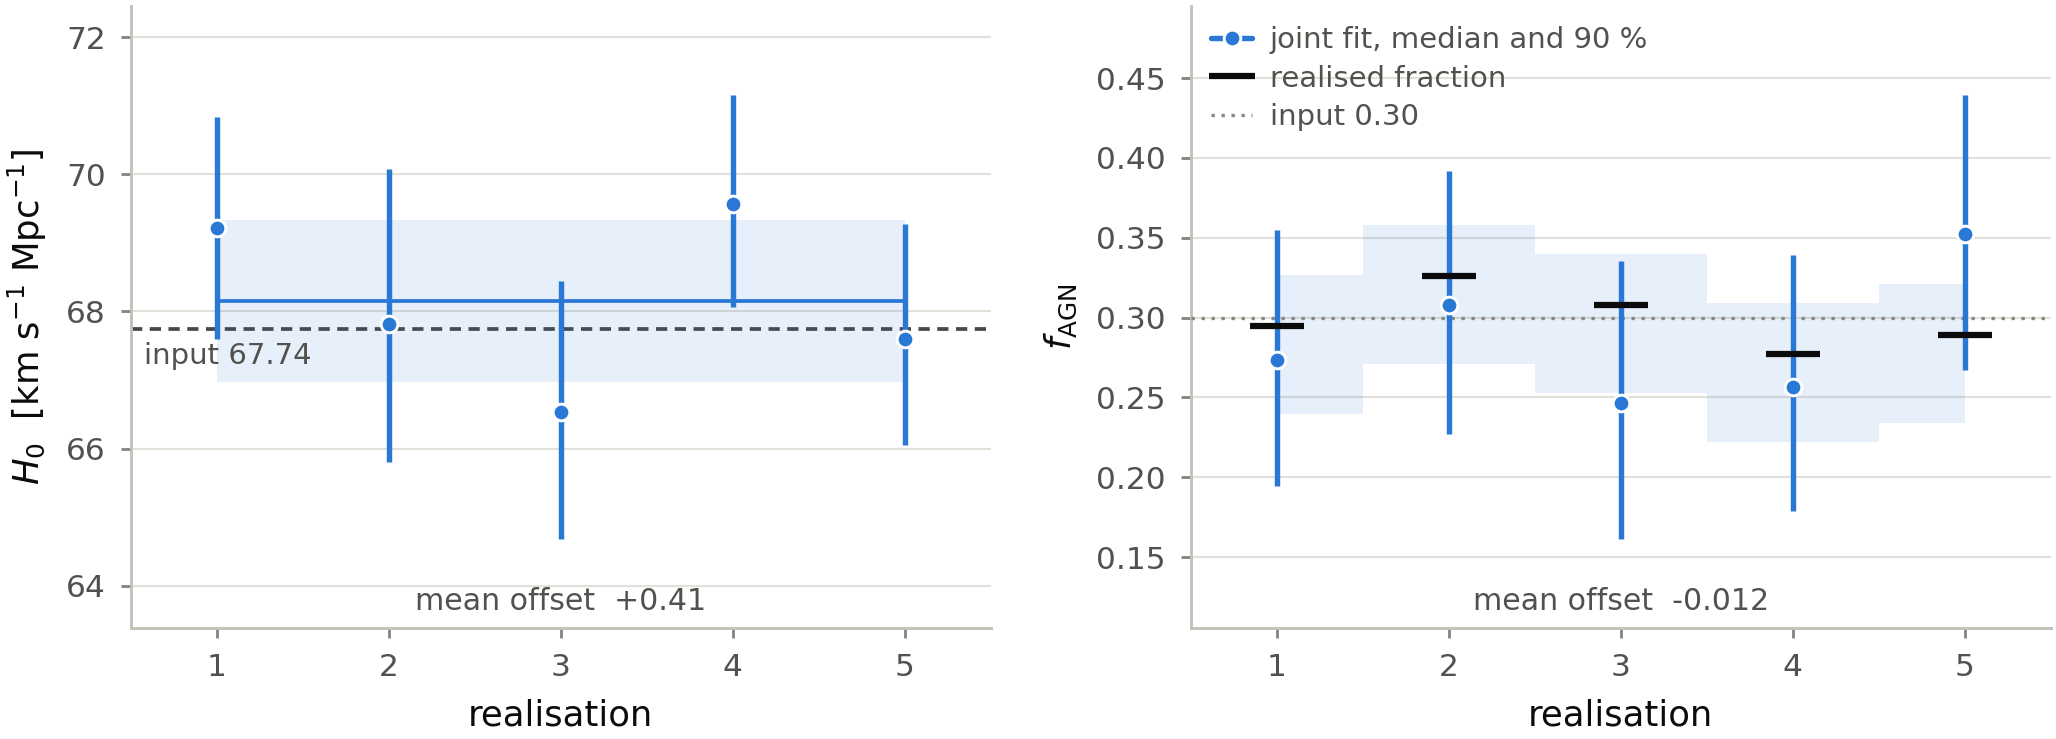
\includegraphics[width=\textwidth]{figures/fig_closure.pdf}
\caption{The joint measurement repeated on \ClosureNseeds\ independent
realisations of the simulated universe, each with its own density field,
catalogs and \EvNobs\ events. Points and bars are per-realisation medians
with 90\% intervals; the shaded band is the 90\% interval on the mean offset
over the \ClosureNseeds\ realisations. Left: \Hz\ against the input value
(mean offset $\ClosureHzero$~\kmsmpc). Right: \fagn\ against each
realisation's own realised hosted fraction (black ticks; mean offset
$\ClosureFagnReal$); the band steps because the reference differs per
realisation, and the dotted line is the input probability \FagnTruthPlanted.
The mean offsets are consistent with zero.
\label{fig:closure}}
\end{figure*}

The measurement of \S\ref{sec:results:joint} rests on one realisation of
every random step in \S\ref{sec:data}: the density field, the catalogs
drawn from it, the hosts, the measurements, and the injection sets. We
repeat the entire construction \ClosureNseeds\ times with independent draws
and repeat the joint measurement on each (Figure~\ref{fig:closure}). The
mean offsets are consistent with zero.

The mean offset of \Hz\ from the input value is $\ClosureHzero$~\kmsmpc,
and the mean offset of \fagn\ from each realisation's own hosted fraction is
$\ClosureFagnReal$ ($\ClosureFagnPlanted$ against the input probability).
The input values fall inside the 68\% intervals in
\ClosureHzeroInSixtyEight\ of \ClosureNseeds\ realisations for \Hz\ and
\ClosureFagnInSixtyEight\ for \fagn, and inside the 90\% intervals in
\ClosureHzeroInNinety\ and \ClosureFagnInNinety, consistent with the
nominal rates for \ClosureNseeds\ draws. The realisation-to-realisation
scatter of the \Hz\ medians is \ClosureScatterHzeroRatio\ times the mean
quoted half-width (\ClosureScatterFagnRatio\ for \fagn), so the quoted
intervals are honest to the precision \ClosureNseeds\ realisations can test.
The matched-host controls of \S\ref{sec:results} also recover across
realisations, with mean offsets of $\CtrlGalMean$~\kmsmpc\ (galaxies; the
input value inside the 68\% interval in \CtrlGalInSixtyEight\ of
\CtrlNseeds\ realisations and inside the 90\% in \CtrlGalInNinety) and
$\CtrlAgnMean$~\kmsmpc\ (AGN; \CtrlAgnInSixtyEight\ of \CtrlNseeds\ at 68\%
and \CtrlAgnInNinety\ at 90\%). The correlation between the two parameters
stays small across realisations, $\rho = \JointRhoMean$.

\PureNseeds\ realisations measure not only whether the single-catalog
analyses of \S\ref{sec:results:single} recover the input value but how wide
their intervals should be, and the two tracers answer differently. The
realisation-to-realisation scatter of the galaxy medians is \EnsGalRatio\
times the mean quoted 68\% half-width, so the galaxy interval is the size it
claims to be. The AGN interval is not. Its scatter is \EnsAgnRatio\ times the
quoted half-width, and its coverage sits below the diagonal across the whole
range of credible levels in Figure~\ref{fig:pure}. The matched-host controls
show the same contrast over \EnsCtrlNseeds\ realisations, \EnsCtrlGalRatio\
for galaxies against \EnsCtrlAgnRatio\ for AGN, and those controls divide one
event set by host type rather than drawing a new one, so the deficit follows
the sparse catalog rather than the choice of events. We read it as sample
variance of the sparse catalog itself, which a fit conditioned on the catalog
it was given cannot see; the realisations redraw catalogs and events together,
so they do not separate that from variance in which events are detected.
Inflating each tracer's half-width by its own measured factor moves the sparse
catalog's advantage at equal event count from $\PureWidthRatioPerSeed$ to
\EnsWidthRatioCorrected\ in the ratio of half-widths. The sparse catalog still
carries more information per event that belongs to it; what moves is how much.

The free-density flux-limited fit replicates as well. Repeated on
\NSeedsIncomplete\ independent
realisations at the shallowest limit, it stays within
\GalAnchorOffsetMaxDex~dex of the input galaxy
density, with the input value inside the 68\% interval in every realisation.
In each the data prefer the luminosity-function completeness over the
number-count completeness by at least \SeedLnBFmin\ $e$-folds
(\S\ref{sec:results:incomplete}).

With \Hz\ held at its input value, the events as observed give
$\fagn = \FagnRecord$ (68\% interval \FagnRecordCi), and permuting the
observed sky positions among the events, so that every event keeps its
distance and its localisation area but no longer points at its own host,
collapses the recovered fraction to \FagnNull\ (\FagnNullCi). The
observed-sky value lies far outside the permuted data's 90\% range,
\FagnNullCiNinety, so host association, not the catalogs' global structure,
carries the measurement.

The mixture likelihood contains both single-catalog analyses as its
endpoints: at $\fagn = 0$ and $\fagn = 1$ its likelihood and its selection
integral reduce to the single-catalog ones, and the evaluated posteriors
reproduce the measurements of \S\ref{sec:results:single} to machine
precision. An injection set drawn independently of the
catalogs, from the source population and the comoving volume alone,
reproduces the joint medians: $\Hz = \HzeroJointCross$ against
\HzeroJointMedian~\kmsmpc\ on a 68\% width of \HzeroJointWidth, and
$\fagn = \FagnJointCross$ against \FagnJointMedian\ on a width of
\FagnJointWidth. Finally, the detectable fraction $\mu(\Lambda)$ of
Equation~(\ref{eq:mu}) is a Monte Carlo estimate, and its error moves every
event coherently rather than averaging away. The error of the mixture's own
term is not measured directly, but its $\fagn = 0$ and $\fagn = 1$ limits
bracket it between \SelMcJointLo\ and \SelMcJointHi~\kmsmpc\ per
realisation; carried onto the mean over the \ClosureNseeds\ realisations it
is at most half that mean's standard error.
